
\begin{center}
    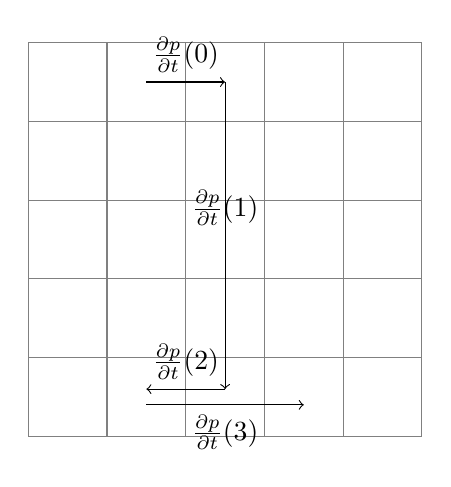
\begin{tikzpicture}
        \draw [step=1,gray,thin] (0,0) grid (5,5);

        \pause
        \draw [->] (1.5, 4.5) -- (2.5, 4.5) node[midway, above] {$\frac{\partial p}{\partial t}(0)$};

        \pause
        \draw [->] (2.5, 4.5) -- (2.5, 0.6) node[midway, above] {$\frac{\partial p}{\partial t}(1)$};

        \pause
        \draw [->] (2.5, 0.6) -- (1.5, 0.6) node[midway, above] {$\frac{\partial p}{\partial t}(2)$};

        \pause
        \draw [->] (1.5, 0.4) -- (3.5, 0.4) node[midway, below] {$\frac{\partial p}{\partial t}(3)$};


    \end{tikzpicture}
\end{center}